\documentclass[a4paper, 12pt]{article}

\usepackage[portuges]{babel}
\usepackage[utf8]{inputenc}
\usepackage{amsmath}
\usepackage{indentfirst}
\usepackage{graphicx}
\usepackage[colorinlistoftodos]{todonotes}
\usepackage{biblatex} %Imports biblatex package
\addbibresource{refs.bib}
%\bibliography{refs}
\usepackage{siunitx}
\usepackage{float}
\usepackage{amsmath,empheq}
\usepackage{systeme,mathtools}
\usepackage{amsmath}
\usepackage{graphicx,subcaption} 
\usepackage{siunitx}
\usepackage{booktabs}
\usepackage{adjustbox}
\usepackage{array}     % Melhor controle de tabelas
\usepackage{tabularx}  % Tabelas com largura ajustável
\usepackage{amsmath}
% parte para escrever em python
\usepackage[T1]{fontenc}
\usepackage{listings}
\usepackage{listingsutf8}
\usepackage[version=4]{mhchem}
\usepackage[acronym]{glossaries} % habilita glossário de siglas
\makeglossaries
\usepackage{xcolor}
\usepackage{setspace}

\definecolor{codegreen}{rgb}{0,0.6,0}
\definecolor{codegray}{rgb}{0.5,0.5,0.5}
\definecolor{codepurple}{rgb}{0.58,0,0.82}
\definecolor{backcolour}{rgb}{0.95,0.95,0.92}

\lstdefinestyle{mystyle}{
    backgroundcolor=\color{backcolour},   
    commentstyle=\color{codegreen},
    keywordstyle=\color{magenta},
    numberstyle=\tiny\color{codegray},
    stringstyle=\color{codepurple},
    basicstyle=\footnotesize,
    breakatwhitespace=false,         
    breaklines=true,                 
    captionpos=b,                    
    keepspaces=true,                 
    numbers=left,                    
    numbersep=5pt,                  
    showspaces=false,                
    showstringspaces=false,
    showtabs=false,                  
    tabsize=2,
    %literate={á}{{\'a}}1 {ã}{{\~a}}1 {é}{{\'e}}1 {ç}{{\c{c}}}1 {Ç}{{\c{C}}}1
    literate={é}{{\'{e}}}1 {è}{{\`{e}}}1 {ê}{{\^{e}}}1 {ë}{{\¨{e}}}1 {É}{{\'{E}}}1 {Ê}{{\^{E}}}1 {û}{{\^{u}}}1 {ù}{{\`{u}}}1 {â}{{\^{a}}}1 {à}{{\`{a}}}1 {á}{{\'{a}}}1 {ã}{{\~{a}}}1 {Á}{{\'{A}}}1 {Â}{{\^{A}}}1 {Ã}{{\~{A}}}1 {ç}{{\c{c}}}1 {Ç}{{\c{C}}}1 {õ}{{\~{o}}}1 {ó}{{\'{o}}}1 {ô}{{\^{o}}}1 {Õ}{{\~{O}}}1 {Ó}{{\'{O}}}1 {Ô}{{\^{O}}}1 {î}{{\^{i}}}1 {Î}{{\^{I}}}1 {í}{{\'{i}}}1 {Í}{{\~{Í}}}1 {°}{\textdegree}1, 
}
 
\lstset{style=mystyle}


% Note that the sign must be
%  µ
%  MICRO SIGN
%  Unicode: U+00B5, UTF-8: C2 B5
% and \emph{not}
%  μ
%  GREEK SMALL LETTER MU
%  Unicode: U+03BC, UTF-8: CE BC
\sisetup{math-micro=\text{µ},text-micro=µ}

%title{Experiência 3: Máquinas Síncronas}

%author{Caio Rosa \\ João Antônio do Amarante \\ Rodrigo \\ Thuane}

%\date{\today}
\setlength {\marginparwidth }{2cm}
\usepackage{hyperref}
\hypersetup{
    colorlinks=true,
    linkcolor=blue,
    filecolor=magenta,      
    urlcolor=cyan,
    pdftitle={Overleaf Example},
    pdfpagemode=FullScreen,
    }

\urlstyle{same}

\begin{document}
%\maketitle

\begin{titlepage}
	\begin{center}
%		\huge{Universidade de Caxias do Sul}

\vspace{10pt}
\begin{figure}[!ht]
\centering

\includegraphics[width=3.5cm]{logo_ucs.png}
\end{figure}
        
        \vspace{45pt}
        
		\textbf{{\LARGE
                \begin{spacing}{1.2}
            \textbf{Relatório para o módulo de Análise Modal e Dinâmica pelo Método dos Elementos Finitos da Especialização em Simulações Estruturais, Fluidodinâmicas e 
Multicorpos: Instrumentação e Durabilidade}
            \end{spacing}}}
		\vspace{70pt}
		
	\end{center}
	
	\begin{flushleft}
		\begin{tabbing}
			Aluno:\qquad\qquad\= Antonio Victor de Souza Correa \\
			Professor:\> Carlos Aurélio da Silva Carvalho\\
			
		
	\end{tabbing}
		  
	\end{flushleft}
	
	\begin{center}
		\vspace{\fill}
		Rio de Janeiro, Novembro de 2026
	\end{center}
\end{titlepage}
%%%%%%%%%%%%%%%%%%%%%%%%%%%%%%%%%%%%%%%%%%%%%%%%%%%%%%%%%%%
\newpage
\tableofcontents
\thispagestyle{empty}

\newpage
\pagenumbering{arabic}

%%%%%%%%%%%%%%%%%%%%%%%%%%%%%%%%%%%%%%%%%%%%%%%%%%%%%%%%%
%%%%%%%%%%%%%%%%%%%%%%%%%%%%%%%%%%%%%%%%%%%%%%%%%%%%
\section{Introdução}

Este relatório apresenta a resolução da lista de exercícios proposta como avaliação para o módulo de análise modal e dinâmica pelo método dos elementos finitos da especialização em simulações da Universidade Caxias do Sul.

O trabalho compreende três exercícios propostos, com o objetido de relacionar solução analítica, simulação por elementos finitos e interpretação física de sistemas vibratórios. Para a realização das simulações utilizou-se o \textit{software Ansys}.

\section{Exercício 1}

Considere o sistema discreto abaixo, composto por quatro massas ligadas por cinco molas. As 
extremidades são fixas. Dados: m1 = m2 = m3 = m4 = 10 kg; k1 = k2 = k3 = k4 = k5 = 10.000 N/m. Despreze o amortecimento. 

\begin{figure}[H]
    \centering
    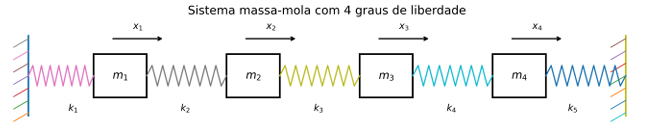
\includegraphics[width=\textwidth, height=7cm, keepaspectratio]{sistema massa mola ex1.png}
    \caption{Sistema massa mola do exercício 1}
    \label{fig:sist massa mola ex1}
\end{figure}

\subsection{Questão A}

\textbf{Identifique os quatro graus de liberdade x1, x2, x3 e x4}.

Os quatro graus de liberdade representam os deslocamentos horizontais independentes de cada massa $m_1, m_2, m_3$ e $m_4$, onde cada uma pode se deslocar para esquerda ou para a direita.

\subsection{Questão B}

\textbf{Monte a matriz de massa global $[M]$ e a matriz de rigidez global $[K]$.}

A matriz de massa global é diagonal:

\begin{equation}
[M] =
\begin{bmatrix}
10 & 0 & 0 & 0 \\
0 & 10 & 0 & 0 \\
0 & 0 & 10 & 0 \\
0 & 0 & 0 & 10
\end{bmatrix}
\ \mathrm{kg}
\label{eq:matriz_massa}
\end{equation}

A matriz de rigidez global é montada com base no acoplamento elástico entre as massas adjacentes:

\begin{equation}
[K] =
\begin{bmatrix}
k_1 + k_2 & -k_2 & 0 & 0 \\
-k_2 & k_2 + k_3 & -k_3 & 0 \\
0 & -k_3 & k_3 + k_4 & -k_4 \\
0 & 0 & -k_4 & k_4 + k_5
\end{bmatrix}
=
\begin{bmatrix}
20.000 & -10.000 & 0 & 0 \\
-10.000 & 20.000 & -10.000 & 0 \\
0 & -10.000 & 20.000 & -10.000 \\
0 & 0 & -10.000 & 20.000
\end{bmatrix}
\label{eq:matriz_rigidez}
\end{equation}

\subsection{Questão C}

\textbf{Escreva a equação do movimento livre: $[M]{\ddot{x}} + [K]{x} = {0}$.}

Em forma matricial, a equação de movimento para vibração livre não amortecida é dada por

\begin{equation}
[M]\{\ddot{x}\} + [K]\{x\} = \{0\}
\label{eq:equacao_movimento}
\end{equation}

substituindo as matrizes de rigidez e massa:

\begin{equation}
\begin{bmatrix}
10 & 0 & 0 & 0\\
0 & 10 & 0 & 0\\
0 & 0 & 10 & 0\\
0 & 0 & 0 & 10
\end{bmatrix}
\begin{Bmatrix}
\ddot{x}_1\\
\ddot{x}_2\\
\ddot{x}_3\\
\ddot{x}_4
\end{Bmatrix}
+
\begin{bmatrix}
20000 & -10000 & 0 & 0\\
-10000 & 20000 & -10000 & 0\\
0 & -10000 & 20000 & -10000\\
0 & 0 & -10000 & 20000
\end{bmatrix}
\begin{Bmatrix}
x_1\\
x_2\\
x_3\\
x_4
\end{Bmatrix}
=
\begin{Bmatrix}
0\\
0\\
0\\
0
\end{Bmatrix}
\label{eq:movimento_livre}
\end{equation}

\subsection{Questão D}

\textbf{Assumindo ${x(t)} = {\phi}e^{(i\omega t)}$, obtenha o problema de autovalores: $([K] - \omega^2[M]){\phi} = {0}$.}

Tomando a solução harmônica ${x(t)} = {\phi}e^{(i\omega t)}$ e derivando duas vezes em relação ao tempo para substituir na equação do movimento livre, temos:

\begin{equation}
\{\ddot{x}(t)\} = -\omega^2 \{\phi\} e^{i\omega t}
\label{eq:aceleracao_harmonica}
\end{equation}

Substituindo na equação do movimento:

\begin{equation}
-\omega^2 [M]\{\phi\} e^{i\omega t}
+ [K]\{\phi\} e^{i\omega t} = \{0\}
\label{eq:substituicao_movimento}
\end{equation}

Colocando o exponencial em evidência:

\begin{equation}
\left([K] - \omega^2[M]\right)
\{\phi\} e^{i\omega t} = \{0\}
\label{eq:fatoracao_movimento}
\end{equation}

Como $e^{i\omega t} \neq 0$, temos:

\begin{equation}
\left([K] - \omega^2[M]\right)\{\phi\} = \{0\}
\label{eq:problema_autovalores}
\end{equation}


\subsection{Questão E}

\textbf{Resolva $det([K] - \omega^2[M]) = 0$ e determine os quatro autovalores, frequências naturais em Hz e 
autovetores.}

\begin{equation}
    \det\left([K] - \omega^2[M]\right) = 0
\end{equation}

Substituindo as matrizes:

\begin{equation}
\begin{vmatrix}
20000 - 10\omega^2 & -10000 & 0 & 0 \\
-10000 & 20000 - 10\omega^2 & -10000 & 0 \\
0 & -10000 & 20000 - 10\omega^2 & -10000 \\
0 & 0 & -10000 & 20000 - 10\omega^2
\end{vmatrix}
= 0
\end{equation}

Dividindo todos os termos por 10 e substituindo $\omega^2$ por $\lambda$:

\begin{equation}
\begin{vmatrix}
2000 - \lambda & -1000 & 0 & 0 \\
-1000 & 2000 - \lambda & -1000 & 0 \\
0 & -1000 & 2000 - \lambda & -1000 \\
0 & 0 & -1000 & 2000 - \lambda
\end{vmatrix}
= 0
\end{equation}

Resolvendo o determinantes encontramos o polinômio:

\begin{equation}
\lambda^4 - 8000\lambda^3
+ 21\,000\,000\lambda^2
- 20\,000\,000\,000\lambda
+ 5\,000\,000\,000\,000 = 0
\end{equation}

Resolvendo o polinômio encontramos os autovalores e em seguida as frequências naturais:


\begin{equation}
\begin{aligned}
\lambda_1 &= 381{,}96 \rightarrow 19,54 rad/s \rightarrow 3,11 Hz\\
\lambda_2 &= 1381{,}96 \rightarrow 37,17 rad/s \rightarrow 5,92 Hz\\
\lambda_3 &= 2618{,}03 \rightarrow 51,16 rad/s \rightarrow 8,14 Hz\\
\lambda_4 &= 3618{,}03 \rightarrow 60,15 rad/s \rightarrow 9,57 Hz
\end{aligned}
\end{equation}

Substituindo os autovalores no problema de autovalores e autovetor \ref{eq:problema_autovalores}:

\begin{equation}
    \left([K] - \lambda_r[M]\right)\{\phi_r\} = \{0\}
\end{equation}

Substituindo as matrizes

\begin{equation}
\begin{bmatrix}
2000-\lambda_i & -1000 & 0 & 0\\
-1000 & 2000-\lambda_i & -1000 & 0\\
0 & -1000 & 2000-\lambda_i & -1000\\
0 & 0 & -1000 & 2000-\lambda_i
\end{bmatrix}
\begin{Bmatrix}
\phi_{1,i}\\
\phi_{2,i}\\
\phi_{3,i}\\
\phi_{4,i}
\end{Bmatrix}
=
\begin{Bmatrix}
0\\
0\\
0\\
0
\end{Bmatrix}
\label{eq:resolvendo autovetores}
\end{equation}

Resolvendo para o primeiro autovalor e adotando $\phi_{1,1} = 1$, temos o primeiro autovetor:

\begin{equation}
\{\phi_1\} =
\begin{Bmatrix}
1 \\
1{,}618 \\
1{,}618 \\
1
\end{Bmatrix}
\end{equation}

Do mesmo modo, para os demais autovetores:

\begin{equation}
\{\phi_2\} =
\begin{Bmatrix}
1 \\
0{,}618 \\
-0{,}618 \\
-1
\end{Bmatrix}
\end{equation}

\begin{equation}
\{\phi_3\} =
\begin{Bmatrix}
1 \\
-0{,}618 \\
-0{,}618 \\
1
\end{Bmatrix}
\end{equation}

\begin{equation}
\{\phi_4\} =
\begin{Bmatrix}
1 \\
-1{,}618 \\
1{,}618 \\
-1
\end{Bmatrix}
\end{equation}

Ortonormalizando os autovetores em relação a massa através da equação \ref{eq: ortonormal}, temos:

\begin{equation}
\{\Phi_i\} =
\frac{\{\phi_i\}}
{\sqrt{\{\phi_i\}^{T}[M]\{\phi_i\}}}
\label{eq: ortonormal}
\end{equation}

\begin{equation}
\begin{aligned}
\{\Phi_1\} &=
\begin{Bmatrix}
0{,}11756 \\
0{,}19021 \\
0{,}19021 \\
0{,}11756
\end{Bmatrix}
\qquad
\{\Phi_2\} =
\begin{Bmatrix}
0{,}19021 \\
0{,}11756 \\
-0{,}11756 \\
-0{,}19021
\end{Bmatrix}
\\[1em]
\{\Phi_3\} &=
\begin{Bmatrix}
0{,}19021 \\
-0{,}11756 \\
-0{,}11756 \\
0{,}19021
\end{Bmatrix}
\qquad
\{\Phi_4\} =
\begin{Bmatrix}
0{,}11756 \\
-0{,}19021 \\
0{,}19021 \\
-0{,}11756
\end{Bmatrix}
\end{aligned}
\end{equation}


\subsection{Questão F}

\textbf{Modele o mesmo sistema em um software de elementos finitos usando elementos de mola e massas 
concentradas.}

\subsection{Questão G}

\textbf{Compare as frequências analíticas e numéricas e calcule o erro percentual.}

\subsection{Questão H}

\textbf{Explique por que, em uma análise modal linear clássica sem pré-tensão, uma força externa não é 
necessária para determinar as frequências naturais.}

\section{Exercício 2}

\textbf{Considere uma placa de aço representando um suporte estrutural fixado ao veículo, com as características e condições de contorno apresentadas na tabela \ref{tab:parametros}.}

\begin{table}[H]
    \centering
    \caption{Parâmetros geométricos, propriedades do material e condições de contorno}
    \label{tab:parametros}
    \begin{tabular}{l l}
        \hline
        \textbf{Parâmetro} & \textbf{Valor} \\ \hline \hline
        Comprimento & 500 mm \\ 
        Largura & 80 mm \\ 
        Espessura & 5 mm \\ 
        Módulo de elasticidade $E$ & 210 GPa \\ 
        Coeficiente de Poisson $\nu$ & 0,30 \\ 
        Densidade $\rho$ & 7850 kg/m$^3$ \\ 
        Condição de contorno & Uma extremidade completamente engastada \\ 
        Massa concentrada inicial & 2,0 kg na extremidade livre \\ \hline
    \end{tabular}
\end{table}



\subsection{Etapa A}

\textbf{Determine as cinco primeiras frequências naturais e identifique a característica predominante das 
respectivas formas modais.}

\subsection{Etapa B}

\textbf{Aplique na extremidade livre uma força de excitação do sistema ( seguindo os conceitos que realizados), 
seja uma aceleração unitária. Realize uma varredura de 0 a 300 Hz e obtenha uma FRF de deslocamento 
ou aceleração na extremidade livre.} 

\begin{itemize}
    \item \textbf{Identifique os principais picos da FRF e compare-os com as frequências naturais da análise modal.} 
    \item \textbf{Explique por que um modo pode existir na análise modal e apresentar pico pequeno ou praticamente não aparecer em determinada FRF.}
\end{itemize}

\subsection{Etapa C}

\textbf{Remova a massa concentrada de 2,0 kg, mantendo geometria, material, malha e condições de contorno. 
Repita a análise modal e a FRF.}

\subsubsection{Questão A}

\textbf{A retirada da massa aumentou ou diminuiu as frequências naturais? Justifique com $f_n \propto \sqrt{\frac{k}{m}}$.} 

\subsubsection{Questão B}

\textbf{Todos os modos sofreram a mesma alteração percentual? Explique considerando a posição da massa e a forma modal.} 

\subsubsection{Questão C}

\textbf{Os picos da FRF acompanharam a alteração das frequências modais?}

\subsubsection{Questão D}

\textbf{A retirada de massa necessariamente melhora o comportamento dinâmico? Justifique.}


\section{Exercício 3}

\textbf{Um componente estrutural fixado à carroceria apresenta frequência natural de 48 Hz. O motor opera entre 
1.800 e 3.600 rpm. Considere inicialmente a excitação de 1ª ordem (1X).} 

\subsection{Questão A}

\textbf{Converta a faixa de rotação de rpm para Hz usando $f = rpm/60$.} 

\subsection{Questão B}

\textbf{Determine se a frequência natural de 48 Hz está dentro ou próxima da faixa de excitação 1X.} 

\subsection{Questão C}

\textbf{Determine a rotação para a qual $fexc~=~fn$.}

\subsection{Questão D}

\textbf{Explique fisicamente o que pode ocorrer quando $fexc~\approx~fn$ e relacione com ressonância.} 

\subsection{Questão E}

\textbf{Discuta possíveis consequências: amplificação de deslocamentos, tensões dinâmicas, ruído, 
desconforto, afrouxamento de uniões, fadiga e falha.} 

\subsection{Questão F}

\textbf{Proponha pelo menos quatro modificações de projeto capazes de afastar o sistema da condição crítica.} 

\subsection{Questão G}

\textbf{Repita a avaliação considerando ordens 1X, 2X e 3X, usando $fexc~=~n\cdot~rpm/60$.} 

\subsection{Questão H}

\textbf{Explique por que conhecer apenas a frequência natural não é suficiente para afirmar que haverá um 
problema de vibração.}

\section{Conclusão}

-ESCREVER

\printbibliography[heading=bibintoc,title={Referências}]



\end{document}